\documentclass[10pt,aspectratio=169]{beamer}
\usetheme{default}\usecolortheme{seagull}\setbeamertemplate{navigation symbols}{}\setbeamertemplate{footline}[frame number]
\usepackage[T1]{fontenc}\usepackage{mathptmx}\usepackage{booktabs}\usepackage{graphicx}\usepackage{tabularx}\usepackage{ragged2e}
\setbeamerfont{title}{size=\large,series=\bfseries}\setbeamerfont{frametitle}{size=\normalsize,series=\bfseries}\setbeamercolor{frametitle}{fg=black}\setbeamercolor{title}{fg=black}
\title{Compiling for a device that keeps moving}\subtitle{Placement and routing at 78.5 against a 283.5 baseline, and what the compiled circuit is worth at run time}
\author{Matthew Stanley Leibel \quad TrueLoop Compute (NEOTECH Inc.)}\date{QSITE 2026 Quantum Coalition, Computational Track}
\begin{document}
\begin{frame}\titlepage\centering\small\textit{A routed circuit is a compile-time object. What a user gets is its success on a device that has drifted since it was characterized.}\end{frame}
\begin{frame}{1. The solver}\small
\textbf{The rules decide the design.} The 2Q list must be reproduced exactly, in order; only SWAPs and the placement are free; depth is the ASAP critical path. So: placement, which qubit moves along which path, and SWAPs that ride in idle slots.\\[6pt]
\textbf{Placement:} interaction graph weighted by gate multiplicity (earlier gates count more), simulated annealing over injective placements.\\[4pt]
\textbf{Routing:} gates in order; candidate SWAPs must bring the current gate one step closer (minimum $d{-}1$ SWAPs, no oscillation); chosen by SABRE lookahead over the next 8 gates plus a charge for the ASAP layer the SWAP lands on.\\[4pt]
\textbf{Refinement:} three SABRE reverse passes, 120 restarts over three seeds, exact scorer in the loop, deterministic.\\[4pt]
\scriptsize\begin{tabular}{lrrrr}\toprule benchmark & baseline & ours & SWAPs & depth\\\midrule ghz\_star & 14.0 & 7.0 & 3 & 8\\ chain\_trotter & 15.0 & 4.5 & 0 & 9\\ ladder\_trotter & 35.5 & 6.5 & 3 & 7\\ qaoa\_random & 39.0 & 11.5 & 6 & 11\\ dense\_random & 122.0 & 46.0 & 33 & 26\\ vqe\_layers & 58.0 & 3.0 & 0 & 6 (optimal)\\\midrule total & 283.5 & \textbf{78.5} & & \\\bottomrule\end{tabular}
\end{frame}
\begin{frame}{2. What the circuit is worth at run time}\begin{columns}[T]\begin{column}{0.62\textwidth}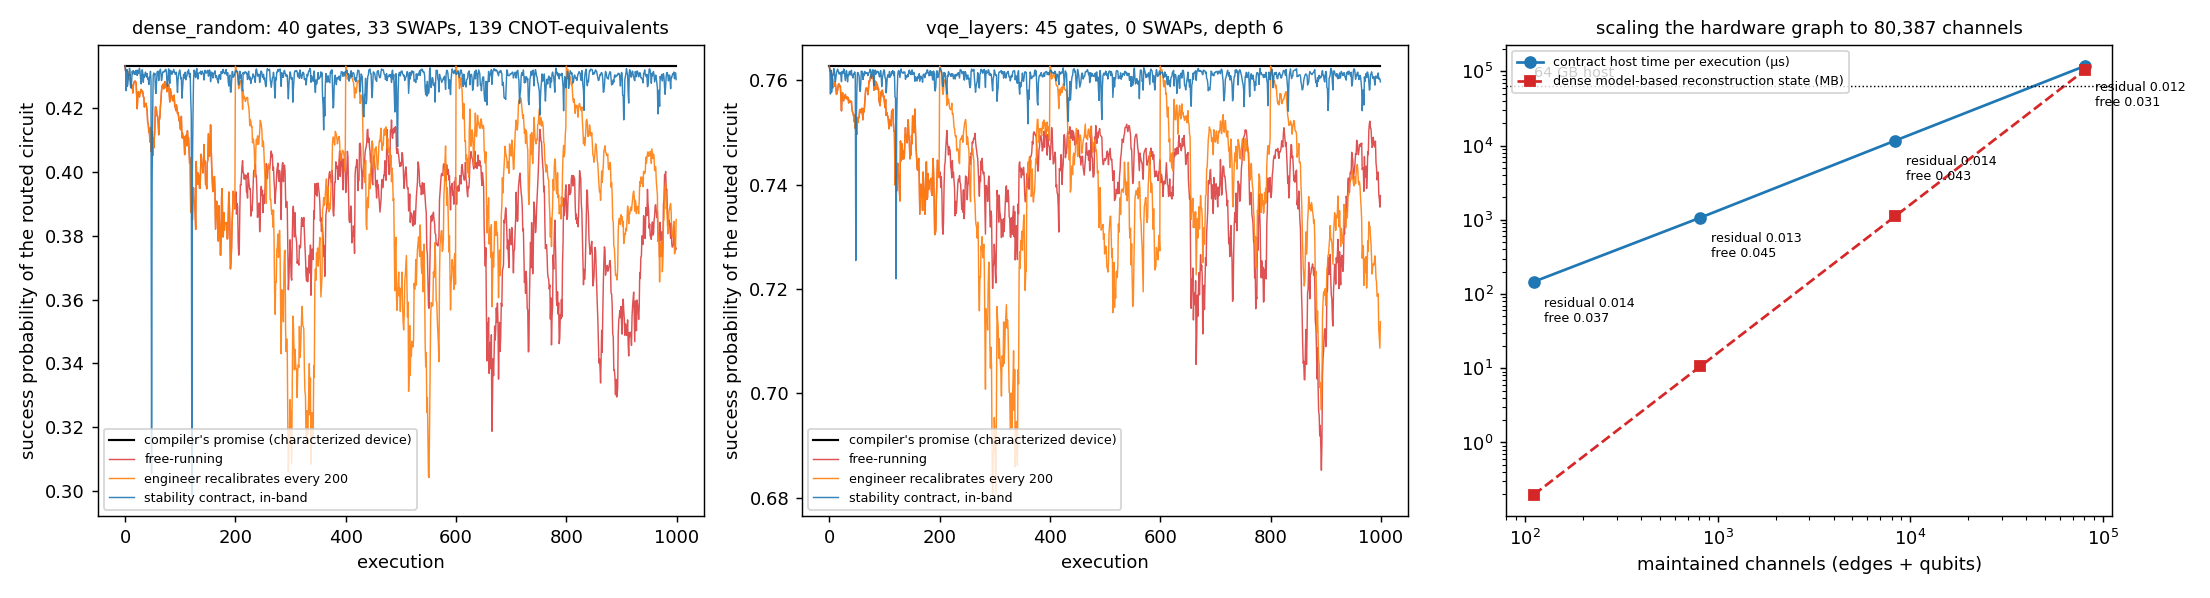
\includegraphics[width=\textwidth]{../figures/runtime_validity.png}\end{column}\begin{column}{0.36\textwidth}\footnotesize
Every edge and qubit drifts after characterization: 4\% wander plus a slow walk. Gate infidelity $= $ floor $+\ \epsilon^2/4$; a SWAP is three CNOTs.\\[6pt]
\textbf{dense\_random, 1,000 executions:} promise 0.433. Free-running ends at 0.373. Engineer every 200: 0.390, dips to 0.304. Contract: \textbf{0.429}, 99\% of the promise, 81\,$\mu$s per execution.\\[6pt]
\textbf{vqe\_layers:} 0.763 promised; contract 0.760.\\[6pt]
The morning re-map exists because the compiler's cost model goes stale. Maintenance keeps it true.
\end{column}\end{columns}\end{frame}
\begin{frame}{3. Why this is the only one that scales}\small
\begin{tabular}{r r r r r}\toprule qubits & channels & contract host / execution & residual (free) & dense reconstruction model\\\midrule 48 & 111 & 146\,$\mu$s & 0.013 (0.037) & 0.2\,MB\\ 336 & 815 & 1.1\,ms & 0.013 (0.045) & 11\,MB\\ 3,360 & 8,319 & 11.6\,ms & 0.014 (0.043) & 1.1\,GB\\ 32,256 & 80,387 & 118\,ms & 0.012 (0.031) & 103\,GB, beyond a 64\,GB host\\\bottomrule\end{tabular}\\[10pt]
Three ways to keep a device where the compiler characterized it. An engineer on standby at every site cannot follow a wander faster than the schedule. Reconstructing the device's state costs $n^2$ memory and $n^3$ setup, and stops at a few thousand channels. An in-band contract is linear in channels and never touches the state.\\[8pt]
\textbf{Honest limits:} a simulated device with measured drift structure, stated floors; the probe rung must be an odd multiple of $\pi/2$ with bounds inside its monotone range, which we learned by breaking it; no Stretch Goal A. The experiment runs as written on hardware: probes are circuits, corrections are angle scales.
\end{frame}
\end{document}
